\documentclass[12pt,a4paper]{report}
\usepackage[top=1cm, bottom=1cm, left=3cm, right=1cm]{geometry}
\usepackage{setspace}
\onehalfspacing
\usepackage {subfigure}
\usepackage {acronym}
\usepackage{multirow}
%\usepackage{psfrag}
% preamble
\usepackage{amsmath}
\usepackage{amsfonts}
\usepackage{amssymb}
\usepackage{anysize}
\usepackage{array}
\usepackage{tabularx}
\usepackage{bbm}
\usepackage{lastpage}
\usepackage{fancyhdr}
\usepackage{tikz}
\usetikzlibrary{calc}
\usepackage[T1]{fontenc}
\usepackage{graphicx}
\usepackage{import}
\graphicspath{ {/} }
\usepackage[english]{babel}
\usepackage{ragged2e}
\usepackage{blindtext}
\usepackage{stfloats}
\usepackage[utf8]{inputenc}


\begin{document}


\begin{center}
\pagenumbering{gobble}
{\Large A Seminar Report}\\
\setstretch{2.00}
{\Large On}
\\
\setstretch{2.00}
{\large \textbf{\lq\lq CROSS-PLATFORM APPLICATION DEVELOPMENT USING REACT NATIVE\rq\rq} }
\\
\setstretch{2.00}
{\Large \textit{By}}
\\
\setstretch{2.00}
{\Large \textbf{Sanket Sabale \\ (Seat No. S190944226)}}
\\
\setstretch{2.00}
{\large \textit{Under the guidance of}}
\\
\setstretch{2.00}
{\Large \textbf{Prof. A. M. Dalvi} }
\\
\setstretch{2.60}
{\Large \textbf{T.E. (COMPUTER ENGINEERING)}}
\\
\setstretch{2.00}
{\large \textbf{2021-22 (Semester I)}}
\\
\setstretch{1.60}
 
\includegraphics[width=0.25\textwidth]{logo}
\\
\setstretch{1.60}
{\large \textbf{DEPARTMENT OF COMPUTER ENGINEERING}}
\\
\setstretch{2.60}
{\small SRTCT's Suman Ramesh Tulsiani Technical Campus - Faculty of Engineering}
\\
\setstretch{2.00}
{\small Old Mumbai - Pune Highway, Khamshet,}
\\
\setstretch{2.00}
{\small Pune, Maharashtra 410405}

\newpage

 
\includegraphics[width=0.15\textwidth]{logo}
\\
\setstretch{1.20}
{\Large SRTCT's Suman Ramesh Tulsiani Technical Campus - Faculty of Engineering}
\\
\setstretch{1.20}
{\small Old Mumbai - Pune Highway, Khamshet,}
\\
\setstretch{1.20}
{\small Pune, Maharashtra 410405}
\\
\setstretch{2.00}
{\large \textbf{DEPARTMENT OF COMPUTER ENGINEERING}}
\\
\setstretch{2.40}
{\LARGE \textit{Certificate}}
\\
\setstretch{2.40}
{\large This is to certify that the seminar report entitled}
\\
\setstretch{2.00}
{\large \textbf{ \textcolor{red}{Cross-Platform Application in React Native}}}
\\
\setstretch{2.00}
{\large Submitted By}
\\
\setstretch{1.80}
{\large \textbf{Sanket Sabale (Seat No. S190944226)}}
\\
\setstretch{1.80}
\begin{FlushLeft}
 is approved by Prof. A. M. Dalvi for submission. It is certified further that, to the
best of my knowledge, the report represents work carried out by my
students as the partial fulfillment for T.E. Computer Engineering
(Semester I) Seminar and Technical communication Laboratory Work as 
prescribed by the University of Pune for the academicyear 2021-22.
\\

\end{FlushLeft}
\begin{figure*}[b]
\begin{tabular}{ c c c }
 \textbf{[ Prof. A. M. Dalvi ]} & \textbf{[ Prof. S. S. Bhoite ]} &  \textbf{[ Prof. A. M. Dalvi ]}  \\ 
 STCL Guide & STCL Co-ordinator & Head of Department     
\end{tabular}
\\
\setstretch{0.80}
\begin{FlushLeft}
{\small Place: Pune }\\
{\small Date: \today }
\end{FlushLeft}
\end{figure*}

\newpage

\pagebreak
\hspace{0pt}
\vfill
{\LARGE \textbf{\textit{Acknowledgement}}}

\begin{FlushLeft}
{\large \textit{
\quad We would like to express our gratitude to all those who helped us to complete
this work. We want to thank our guide Prof. A. M. Dalvi for his continuous help and 
generous assistance. He helped in a broad range of issues from giving us
direction, helping to find the solutions, outlining the requirements and always
having the time to see us.
}}
\\

\end{FlushLeft}

\setstretch{4.00}

\begin{FlushRight}

{\large \textbf{Sanket Sabale}}

\end{FlushRight}



\vfill
\hspace{0pt}
\pagebreak
\end{center}


\newpage 
\pagenumbering{arabic}


%%%%%%%%%%%%%%%% HEADERS N FOOTERS %%%%%%%%%%%%%%%%%%%
\setlength{\headheight}{20pt}
 
\pagestyle{fancyplain}
\renewcommand{\chaptermark}[1]{\markboth{#1}{}}
 
\lhead{\fancyplain{}}
\chead{}
\rhead{\fancyplain{}{\textit{\leftmark}}}
\lfoot{}
%\cfoot{\thepage\ of \pageref{LastPage}}
\cfoot{\thepage}
\rfoot{}

%%%%%%%%%%%%%%%%%%%%%%%%%%%%%%%%%%%%%%%%%%%%%%%%%%%%%%%%%%%%%%%%%%%%%%%%%


\pagenumbering{roman}
\tableofcontents
\newpage

\chapter*{\centering Abstract}


React Native is an Open-Source UI software Framework created by Meta Platforms, in 2015. It is Used to Develop Applications for Android and IOS By enabling developers to use React Framework along with native platform capabilities. It is also being used to develop virtual reality applications at Oculus. The Working Principle of React native are virtually identical to React except that React Native does not manipulate the DOM via the Virtual DOM. It runs in a background process (which  interprets the JavaScript written by the developers ) directly on the end-device and communicates with the native platform via serialized data over an asynchronous and batched bridge. React Components wrap existing native code and interact with native API’s via React’s declarative UI paradigm and JavaScript. While React native styling has a similar sytax to css it does not use HTML or CSS. Instead, messages from the JavaScript thread are used to manipulate native views. React Native also allows developers to write native code in languages such as Java or kotlin for Android, objective-c or swift for ios, and C++/WinRT or  for Windows 10, Which makes it even more flexible Microsoft builds and maintain React Native for windows and React native for macOs.

\newpage

\pagenumbering{arabic}
\chapter{INTRODUCTION}
\section{Introduction}

\hspace{0.5cm} React Native has been successfully adopted by hundreds of businesses worldwide, including Uber, Microsoft, and Facebook, and is used across a whole range of industries. React Native (also known as RN) is a popular JavaScript-based mobile app framework that allows you to build natively-rendered mobile apps for iOS and Android. The framework lets you create an application for various platforms by using the same codebase. React Native was first released by Facebook as an open-source project in 2015. In just a couple of years, it became one of the top solutions used for mobile development. React Native development is used to power some of the world’s leading mobile apps, including Instagram, Facebook, and Skype. We discuss these and other examples of React Native-powered apps further in this post. When Facebook first decided to make its service available on mobile devices, instead of building out a native app like many top tech players at the time, they decided to run with a mobile webpage based on HTML5. However, the solution didn’t stand the test of time, leaving much room for UI and performance improvements. In fact, in 2012, Mark Zuckerberg admitted that “the biggest mistake we made as a company was betting too much on HTML as opposed to native.”

\section{Scope of work}
\hspace{0.5cm} A React Native developer is a highly skilled individual who can create well-structured front-end architecture, APIs, and can also write reusable, and scalable JavaScript codes. A clear and comprehensive React Native developer job description helps you attract highly skilled engineers to your organization. From making visualizations that can render huge quantities of data to engineer web applications, a skilled React Native developer can handle them all. Companies that wish to have developers who could help them in creating user-facing software solutions, adding new features, and fixing problems must hire the best React Native developer. For now there are typescript is language to write a code in React Native used by many developers so it Basically means React native developers have great future with more resposibilities.




\section{Motivation}
\hspace{0.5cm} Today React Native is Accepted By Many Different Companies and They are Hiring React Native Developers . \\
\begin{figure}[h]
    \centering
    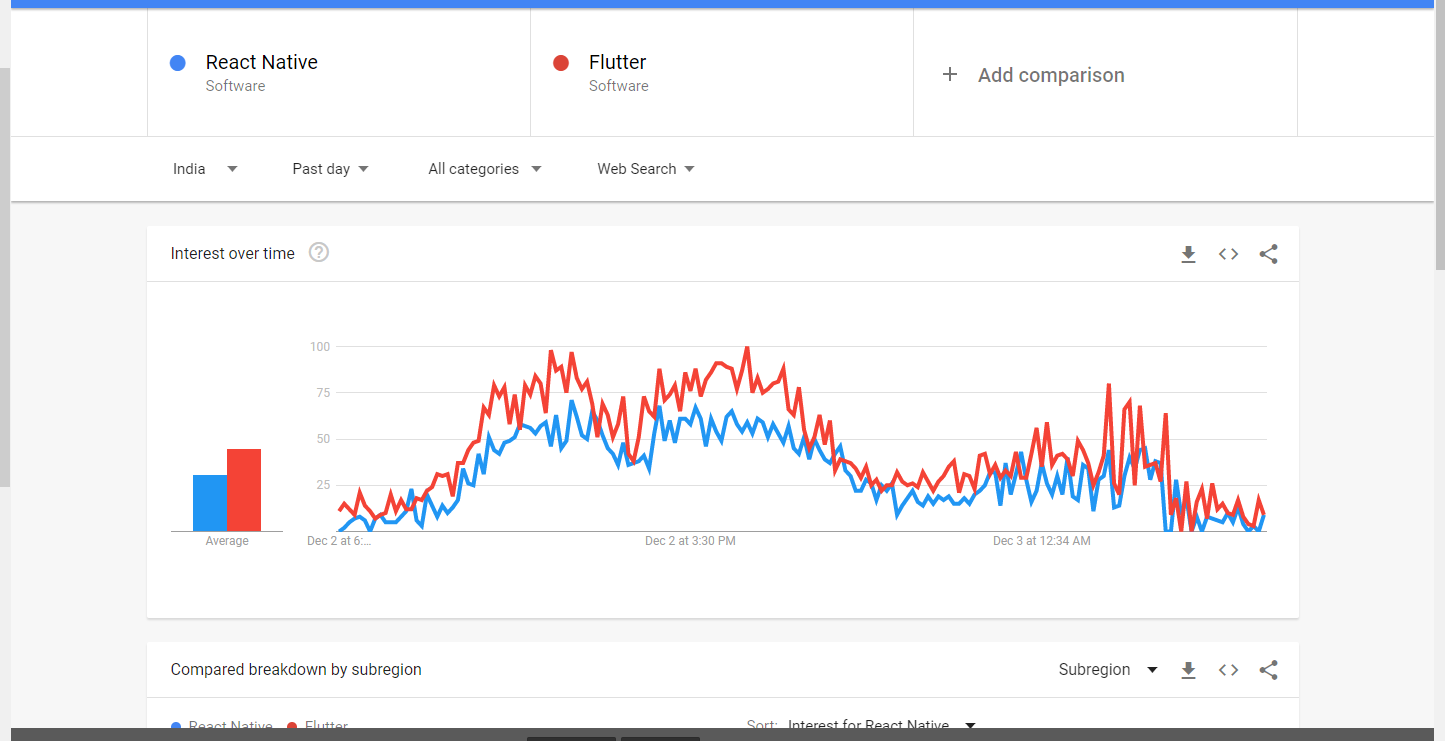
\includegraphics[width=0.85\textwidth]{react_trends}
\caption{React Native Trends}
    \label{fig:1}
\end{figure}
\\
Also React Native is doing a greate job to beat the other alternatives.We all know that Android users are huge as compare to another platforms and thats why there are millions of apps are downloaded every day so demand of an android developers are really big so if you are wanted to become an android developer you need to pick a perticular android technology but if you have knowledge of web development like JS,HTML,CSS and ReactJS You can Continue with it and you can master these development with React Native. It is a Greate Platform who can give you authority to write code once and make or convert it in IOS and Android App so you don't need to write code for android and ios differently so the big problem are going to be fixed up here. React Native is really gone to easy who are in web development you can connect any backend framework to the android app which is build with react native also there are few other tech as well where you can connect backend but in react native it is easy to connect.

\newpage

\chapter{Literature Survey}


\begin{tabular}{ |c | m{2.5cm} | m{2cm}| c | m{2cm} | m{2cm} | c | }

  \hline
  sr.no & Title of Page & Author & Published Year & Finding & Future Scope  \\ 
  \hline
  1 & React Native Based Mobile App for Online Experimentation & Xingwei Zhou etal. &  2020 & IEEE Xplore & Helps Student To  get Practicle Exprerince Through 3D \\
  \hline
  2 & React Native Supplements & Paul etal. &  2019 & Springer & Guide For Developers \\ 
\hline
    3 &  Mobile Development in Swift, Java and React Native & Hugo Brito etal. &  2019 & IEEE Xplore & Comparing Technologies \\
\hline 
 4 &  JavaScript in Mobile Applications: React native vs Ionic vs NativeScript vs Native Development & Anabela Gomes etal. &  2018 & IEEE Xplore & Comparing Technologies \\
\hline 

\end{tabular}
\\
\\

\newpage
\begin{tabular}{ |c | m{2.5cm} | m{2cm}| c | m{2cm} | m{2cm} | c | }

  \hline
  sr.no & Title of Page & Author & Published Year & Finding & Future Scope  \\ 
  \hline
 5 &  Exploration of React Native Framework in designing a Rule-Based Application for healthy lifestyle education & Anik Hanifatul Azizah etal. &  2021 & IEEE Xplore & Lifestyle and Education \\
\hline 

 6 &  Implementation of Gamification Octalysis Method at Design and Build a React Native Framework Learning Application & Andre Julian Irawan etal. &  2021 & IEEE Xplore & Research Development \\
\hline
\end{tabular}

\begin{enumerate}
	 {\bf\item  Xingwei Zhou,\lq\lq React Native Based Mobile App for Online Experimentation: Helps Student To  get Practicle Exprerince Through 3D\rq\rq,IEEE, 2020}\\
\\
In These Article We Found That Author is Telling us That How a Laboratory can be an online tool for everyones use by react native so basically The Concept is there are so many collages which don't have 
practical lab so we can create an app for those student so that he can practice on 3D images and Touchable Effects its looks similar to real practice in it so we can solve a problem of Practical labs in all collages but there some things That i like to update is that we can improve thos UI for students and every single branch needs there own space for practice it also we can include some of test exams so that teacher can see knowledge of student or What he gain? so far. 

\newpage


{\bf\item Paul,\lq\lq React Native Supplements : Best Guide for Developers who try to create Custom Components\rq\rq,Springer,2019}\\



 These Article is written for help to understand the backend code of React Native. In these Reflux Patterns are explained in very different and Easier manar so that if react native developers whants to implement somethings they get help from these pattern not only these article also tells about Redux the big state management tools to manage states Many of the industries are actually working on it.
So These Articles also tells about how to use redux? How the you can debugg your apps in android phone using deugging mode. But we can implement some libraries for easy development and we can import statements to import more packets. There are lots of things are covered in these article and its helpfull when wants to understand React native deep concepts but for now we have lot more libraries that comes with pre-builted code that help us to us functionality directly on our App. 


{\bf\item Hugo Brito,\lq\lq Mobile Development in Swift, Java and React Native: Comparing Different Technologies with React Native\rq\rq , IEEE, 2019}\\

 We know that there are so many technologies are present in the market for creating Android and IOS apps but which is best and how we can found it? The perticular question is solved in these article. while we are creating a Native App we are using Java For android and swift for IOS and to create a both platform application we are using React Native. In native application we found that the performnce of it is really good as compaire to react native but to use more and different library  we need to write to much heavy code and these may be possible that library not presented so we need to manage lots more things to get that functionality done in native apps so that React native solve our problem my suggestion will be like go for react native its saves your time for writing the code which already present and we can compair with these react native with some more cross-plaforms like flutter  and Ionic. 

\newpage

{\bf\item Anabela Gomes,\lq\lq JavaScript in Mobile Applications: React native vs Ionic vs NativeScript vs Native Development\rq\rq, IEEE, 2018}
\\

 These Article Also Compare React native with other technologies but Its Compare with cross-platforms mean the other platforms also work as like a react native and by these comparison we are getting best idea to which tech is used for what kind of projects? and you can pick a grate platform. In lot more cases the tech you pick is not suitable for that perticular project may be the other tech performs better then your's in that case you need to use another tech for it that explaination is inside these article but my opinion will be to improve or add other platforms to like flutter and again compare with it because flutter is also a greate tool it usages a dart programming language and its more over an object oriented programming language  so the code you are writing is in classes and object its not a functional base thats the big disadvantage of flutter but its also quite popular in the market now.


{\bf\item Anik Hanifatul Azizah,\lq\lq Exploration of React Native Framework in designing a Rule-Based Application for healthy lifestyle education \rq\rq, IEE, 2021}
\\
As  we know in these world is Going to faster tech world and now healthy lifestyles is going to be little bit hard for us to find so that these article tells us how we can live a helthy life styles using React Native Rule-Based Application these application comes with some basic rools so that excising and drinking and some more task can be done throught out the notification functionality and some more functionality so that lifestyle becomes technical healthy. But After read these article i think that there are more things we can improve on to it like exerise videos and basic audio file for stress free brain and some more things but all the way these is greate things to work on it and for the healthy lifestyle these ideal is greate to work on it.


{\bf\item Andre Julian Irawan,\lq\lq Implementation of Gamification Octalysis Method at Design and Build a React Native Framework Learning Application \rq\rq,IEEE, 2021}
\\
This research aims to design and build a React Native learning application using the Octalysis gamification method and measuring the level of behavioral intention to use and immersion of the application based on Hedonic Motivation System Adoption Mode (HMSAM). Application testing is carried out by field testing to user who wants to learn React Native. Questionnaire that has been created referring to HMSAM model to measure intrinsic motivation of the user such as user's desire to use the application again (behavioral intention to use) and user focus when using the application (immersion). Evaluation result shows that users strongly agree that they are going to use the React Native learning application in the future with average percentage of 83,24 percentage and users agree that they feel focus when using the React Native learning application with average percentage of 73,79 percentage.
\end{enumerate}
\newpage

\chapter{Proposed System}
\section{Problem Statement}
 In real industries we found that when application project started client requirement is App should be work on cross-plaforms means it can able to run on android as well as ios devices so if you try to understand this thing is little bit complecated for development first developers needs to write code for android and then he also need to write there codes for ios in both different languages so company need to hire developers for android as well as ios so that he can complete the clients project in efficient manor but some how the features which you see in IOS not available in Android in that case android appx become littel bit different from ios app not the UI but feature are different and thats the big reason for big compnies are switching to cross-platform development I am not saying that cross-platform is best that other native platforms there is advantages  of native platforms as well but with the cross-platform application companies can save his time also they don't need hire different developers for different platforms so its saves money as well. There are some Companies who are working on native platforms as well because not every client say i need cross-platform apps some clients are only need android app to be developed in that case to make app more fast companies prefer to go for native platforms like Kotlin or Java. Also Same as IOS developers they work on objective-c and Swift for creating apps for IOS devices so companies are also hire them as well now why companies is are hiring native developers? if the cross-platform technology is here? as i said native apps have there own advantages like you can customize everything which you like and create interface as you want.

\newpage

\section{System Architechture}
\begin{figure}[h]
    \centering
    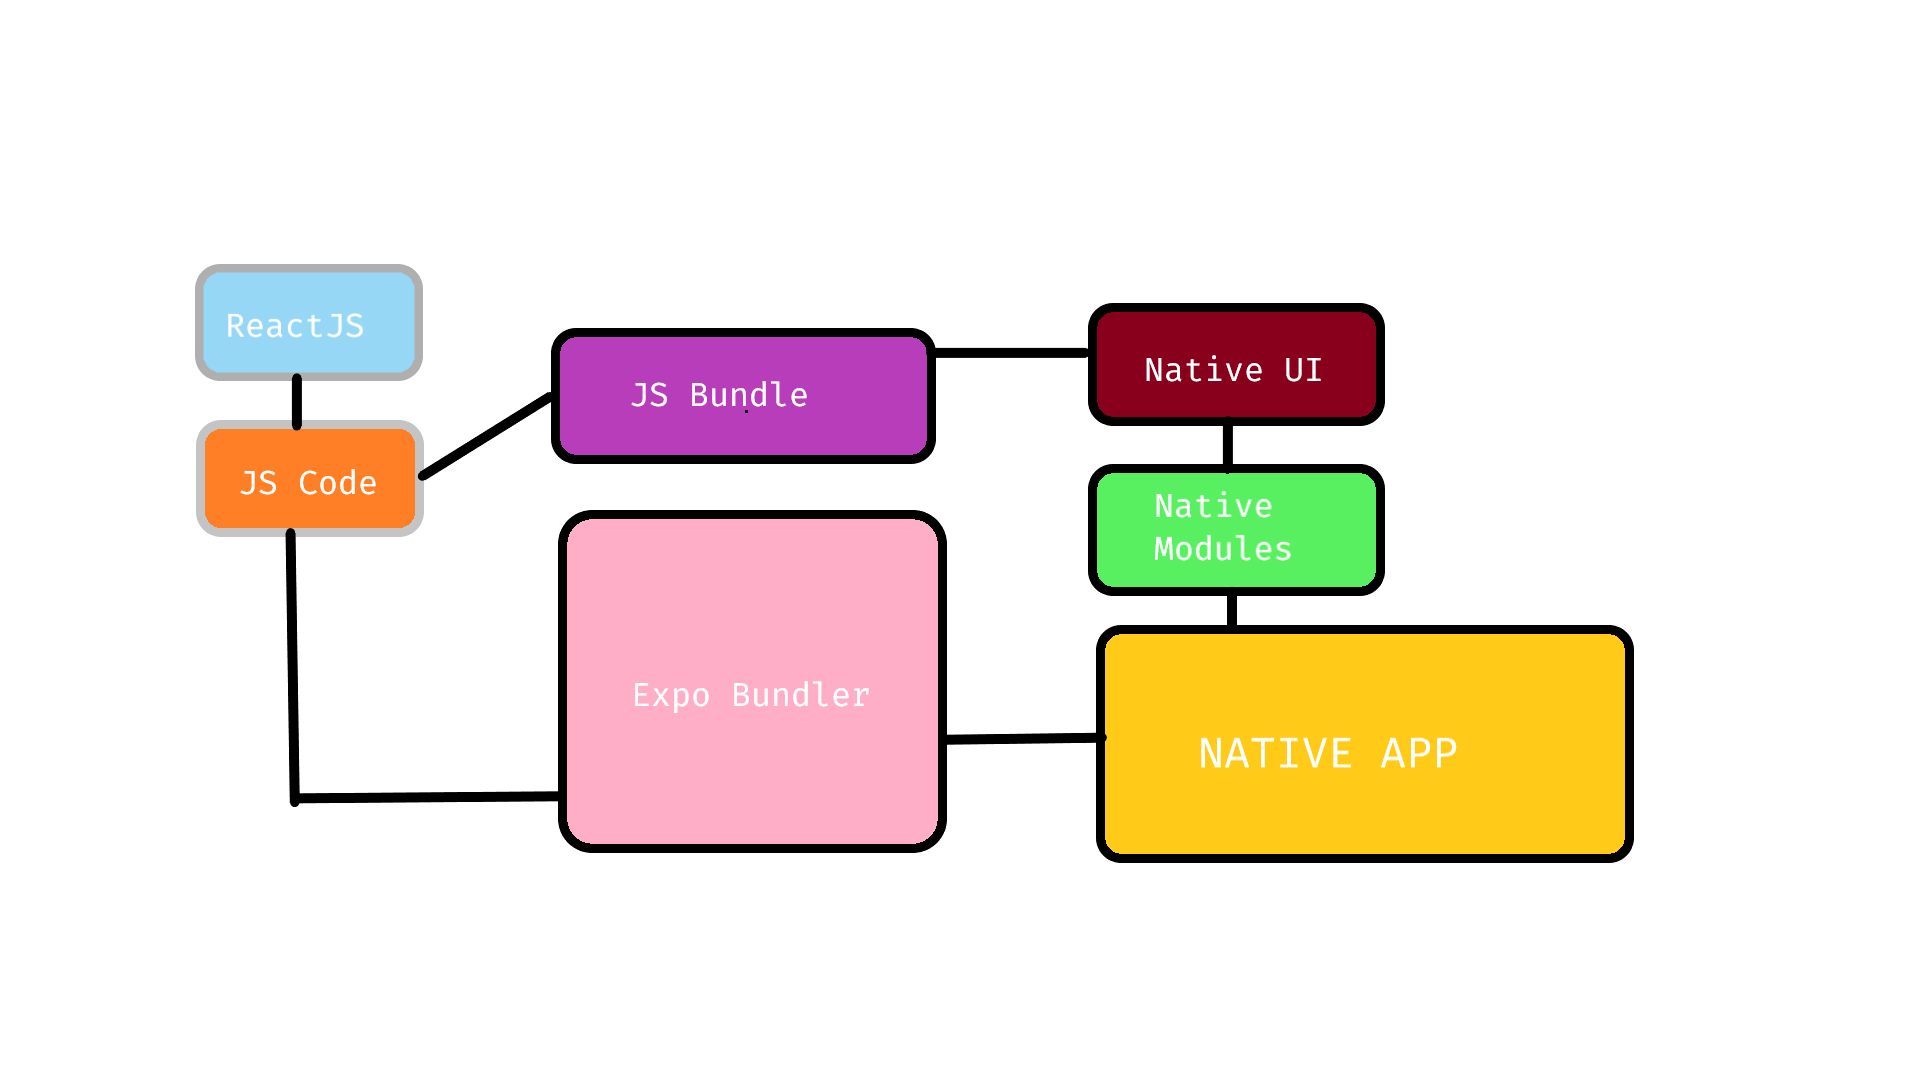
\includegraphics[width=0.75\textwidth]{arch}
\caption{Architecture}
    \label{fig:1}
\end{figure}
 React Native is a good solution if you’re looking for a way to build a scalable application that would run on several platforms fast. Thus, you can start with an MVP, attract the first users, and get to the market earlier than your competitors manage to do the same. As for now, it remains the core tech for building cross-platform software. However, the React Native architecture is not perfect and requires further improvement. If you take a look at React Native layout, you’ll see that the framework uses a Bridge to communicate with native modules, which often creates a queue as these two sides are unaware of each other. Such a process might create performance limitations that negatively affect user experience. To address these and other challenges of the React Native layout, the team introduces regular updates, aiming to streamline developers’ experience. The latest massive update took place on July 6, 2020, when the team at Facebook redesigned the entire error, warning, and log system by introducing an updated LogBox. Such updates are frequent to come. So, if you have React Native in your tech stack, be sure the framework will evolve and become more native and developer-friendly than it was before.

\newpage

\chapter{Methodology}
\section{Algorithm}
\subsection{Diffing algorithm}

Before updating the user interface, React uses a reconciliation algorithm to compare the new tree with the most recent tree to find out the most efficient way to update the user interface. The user interface is not necessary a browser interface but can be android/IOS application (React native or React IOS).

\subsection{Heuristic algorithms}
A heuristic algorithm is one that is designed to solve a problem in a faster and more efficient fashion than traditional methods by sacrificing optimality, accuracy, precision, or completeness for speed. Heuristic algorithms often times used to solve NP-complete problems, a class of decision problems.

\subsection{React Fiber}
React Fiber is a completely backward-compatible rewrite of the old reconciler. This new reconciliation algorithm from React is called Fiber Reconciler. The name comes from fiber, which it uses to represent the node of the DOM tree. We will go through fiber in detail in later sections.

\newpage

\section{Components}
There are some components are built in and it presented in React Native -
\subsection{Basic Components}
In the Basic Components we see basic tags for creating user Interface in our application where you can build some stuff that really makes importance of our app.
\begin{itemize}
  \item View.
  \item Text.
  \item Image.
  \item TextInput.
\end{itemize}

\subsection{Android Components}
We know that react native is based on JS Bundle so to convert JS bundle into real android app you need components Those components are help to achive some basic things in android  we just need to use them in out code. The components are  :- 
\\
\begin{itemize}
  \item BackHandler.
  \item DrawLayoutAndroid.
  \item PermissionsAndroid.
  \item ToastAndroid.
\end{itemize}

\subsection{IOS components}
If in react native android components are present then ios components are also for ios development if we try to create app for both platforms it require to follow every rule of both platforms so that we can achive a best output.

\begin{itemize}
  \item SafeAreaView.
  \item ActionSheetIOS.
\end{itemize}

\newpage

\chapter{Result Analysis}
\section{Comparison of Existing System and Proposed System}
\subsection{ Existing System}
In The React Native we are bundling JS Code and Converting into Java Code for creating android app and the existing system takes more time to do dubugging but yes its also provide a hot reload functionality as well but to do an bundle task its require so much time so that was a big problem? Its Like Restarting bundling, adding more third party library its become so much hard to do in React natives existing system it also takes to much space on our system so it can be little hard say these is greate system to work.

\subsection{Proposed System}
We know in the existing system our time and space both are take high value now i suggest to make in different way by using expo app in these expo app we dont need to worry about bundling things for ios and android its done by the expo app what we need to do is just install expo app connect with our react native project these will save our time and space. for starting point we need to install Expo app on our testing device which may ios or android expo support both platform after that once you run your code application will run on Expo app itself and you will see the result just to debug and create apk file we need to go for server and download some files in expo so that you can get real world app in you system.

\newpage

\section{Advantages}

\subsection{Creating Both Platform Application with Same Code Base}
In React Native World we dont need to learn different programming language for different platform you just need to use javascript and react framwork to create app for both platform thats big advantage of React Native.

\subsection{Reusable Components}
Most Useful feature in ReactJs that also works in React Native where you can create a specific component in different file and that you can use it enywhere where you want  it just lets say you are building a button and you want that button on multiple pages so for that you dont need write code for different pages you just need to put it in one file in functional formate and call into another file where you want that button thats it.


\subsection{ Hot Reload }
Hot Reloading, based on Hot Module Replacement (HMR), was introduced after the first reloading process was conducted. While retaining the features and function sequence, Hot Reloading has an added advantage after saving changes in the file, an HMR intermediator then proceeds to keep the updated files into the required places as the app continues to operate in the background. The primary advantage of using Hot Reloading lies in its ability to sanction changes in the source code in a fashion that lets the developer view the codes, even if he does not recompile the app.

\subsection{Cost-Effective Solution}
The benefit of code reusability offered by React Native helps diminish costs of app creation to a large extent. With this framework, coders need not write separate codes for iOS and Android and can simply code the application in the existing language. This results in the need for a smaller team of native developers for all app development businesses and ensures a sharp reduction in project completion time aided by the competence of the React Native community.

\newpage

\section{Disadvantages}

\subsection{Difficult to Learn}
Learning React Native can be very challenging, especially for freshers in app development who might find creating applications with JSX in the JavaScript syntax extension difficult. Besides React Native, app developers must know native app coding too. React Native libraries with native bridges for features like maps, videos, etc. needs developers with in-depth knowledge, if not expertise, of three platforms. Developers who don’t have the knowledge of multiple platforms can find fixing some inconsistencies in both iOS and Android platforms quite difficult. Hence , the learning curve is steep and may delay development or increase timelines.

\subsection{Low Security}
React Native is a JavaScript library and also an open source framework, due to which developers often face the challenge of keeping the app secure. JavaScript is quite fragile, and this results in some developers experiencing low levels of safety. When making apps that need extra layers of security, such as banking or finance applications, you need to be extra cautious. Otherwise, malicious code snippets can pose a critical threat to the app’s safety features. This is why developers sometimes avoid building financial apps on React Native.

\subsection{Complex UI}
According to many coders, React Native isn’t the right choice for apps that need complex gestures, screen transitions, animations, or require many interactions. Despite React Native having a gesture responder system, coders might continue to struggle with screens with complicated gestures. This is because iOS and Android touch subsystems are so different from each other, that using a unified API might be challenging.

\chapter{Conclution and Future Scope}

\section{Conclution}
\begin{FlushLeft}
{\large React Native has the highest performance among cross-platform frameworks. Apps with this technology have a native look and feel. Indeed, React Native is better and unique than other similar platforms.

It is an excellent framework that is easy to learn and offers good performance as well as an interface that is comparable to native apps. Moreover, some technology enthusiasts consider that react native apps are the future of hybrid mobile apps.

All in all, it’s a win-win game for the organizations that want to satisfy the customers with a tight budget.}
\\

\end{FlushLeft}

\section{Future Scope}

\begin{FlushLeft}
{\large React Native has already become one of the most popular trends for building native, dominant and high-quality mobile applications for both platform iOS and Android. It has gained immense traction for making it possible to build mobile apps that stimulate the performance of native apps. In this digital era, where speed, shortcuts, and fast tools are the need for any mobile application, software programmers giving their best to build mobile apps to run faster with good performance. Interactive user experience and easy development are the significant things that have convinced mobile app developers to work with JavaScript, HTML5, CSS or React Native to build the app. So the Future of react native is great for react developers.}
\\
\end{FlushLeft}

\newpage

\appendix
\chapter{References}
\begin{enumerate}
{\item  Xingwei Zhou,\lq\lq React Native Based Mobile App for Online Experimentation: Helps Student To  get Practicle Exprerince Through 3D\rq\rq,IEEE, 2020}
{\item Paul,\lq\lq React Native Supplements : Best Guide for Developers who try to create Custom Components\rq\rq,Springer,2019}
{\item Hugo Brito,\lq\lq Mobile Development in Swift, Java and React Native: Comparing Different Technologies with React Native\rq\rq , IEEE, 2019}
{\item Anabela Gomes,\lq\lq JavaScript in Mobile Applications: React native vs Ionic vs NativeScript vs Native Development\rq\rq, IEEE, 2018}
{\item Anik Hanifatul Azizah,\lq\lq Exploration of React Native Framework in designing a Rule-Based Application for healthy lifestyle education \rq\rq, IEEE, 2021}
{\item Andre Julian Irawan,\lq\lq Implementation of Gamification Octalysis Method at Design and Build a React Native Framework Learning Application \rq\rq,IEEE, 2021}
\end{enumerate}


\end{document}